\documentclass[10pt]{mypackage}

% sans serif font:
%\usepackage{cmbright,sfmath,bbold}
%\renewcommand{\mathcal}{\mathtt}

%Euler:
\usepackage{newpxtext,eulerpx,eucal,eufrak}
\renewcommand*{\mathbb}[1]{\varmathbb{#1}}
\renewcommand*{\hbar}{\hslash}

%\usepackage{homework}

\pagestyle{fancy} %better headers
\fancyhf{}
\rhead{Avinash Iyer}
\lhead{Mathematical Methods II Notes}

\setcounter{secnumdepth}{0}

\begin{document}
\RaggedRight
\section{Complex Analysis}%
\subsection{Analyticity and Path-Independence in the Complex Plane}%
\subsubsection{Baby's First Complex Function Theory}%
We are interested in functions of the form $f(z)$, where $z = x+iy$ is some complex number. Note that this is specifically different from a function $g\colon \R^2\rightarrow \Omega$ for some domain $\Omega$; in the latter case, we have independent variables $x$ and $y$, while in the former case, we must express $z = x+iy$.\newline

Now, consider a contour integral
\begin{align*}
  \oint_{C}^{} w(z)\:dz &= \oint_{C}w(z)\:\left(dx + idy\right)\\
                        &= \oint_{C}^{} w(z)\:dx + i\oint_{C}w(z)\:dy.
                        \intertext{Taking $A_x = w(z)$ and $A_y = iw(z)$, we have}
                        &= \oint_{C}^{} \mathbf{A}\cdot\:d\vec{\ell}.
                  \intertext{We want to know if this is equal to, by Green's Theorem,}
                        &= \int_{S}^{} \left(\nabla\times \mathbf{A}\right)\:d\mathbf{a},
\end{align*}
and when this integral is zero. Note that $\left(\nabla\times \mathbf{A}\right)\cdot \hat{n} = 0$, so $\pd{A_y}{x} - \pd{A_x}{y} = 0$.\newline

Note that we can take
\begin{align*}
  w(z) &= u(x,y) + iv(x,y),
\end{align*}
where $z = x + iy$.\newline

After a lot of tedious derivation, we get the Cauchy--Riemann equations.
\begin{theorem}[Cauchy--Riemann Equations]
  \begin{align*}
    \pd{u}{x} &= \pd{v}{y}\\
    \pd{v}{x} &= -\pd{u}{y}.
  \end{align*}
\end{theorem}
Furthermore, the Cauchy--Riemann equations guarantee that $w$ is analytic,\footnote{Equal to its Taylor series, also holomorphic.} which leads to Cauchy's theorem.
\begin{theorem}[Cauchy's Theorem]
  If $C$ is a simple closed curve in a simply connected region, then $w$ is analytic if and only if
  \begin{align*}
    \oint_{C}^{} w(z)\:dz &= 0.
  \end{align*}
\end{theorem}
\begin{fact}
The function $w(z)$ is analytic inside the simply connected region $R$ if any of these hold:
\begin{itemize}
  \item $w$ satisfies the Cauchy--Riemann equations;
  \item $w'(z)$ is unique and exists;
  \item $\pd{w}{\overline{z}} = 0$.
  \item $w$ can be expanded in a Taylor series: $w(z) = \sum_{n\geq 0}c_n\left(z-a\right)^n$;\footnote{This is the real definition of analytic.}
  \item $w(z)$ is path-independent everywhere in $R$: $\oint_{C}w(z)\:dz = 0$.
\end{itemize}
\end{fact}
\begin{example}
  Considering $w(z) = z$, we have $u=x$ and $v=y$, so it satisfies the Cauchy--Riemann equations. However, neither $\re\left(z\right)$ nor $\im\left(z\right)$ are analytic, and neither is $\overline{z} = x-iy$.
\end{example}
\begin{remark}
Whenever we say ``analytic at $p$,'' we mean ``analytic in a neighborhood of $p$.''
\end{remark}
Note that since $\C$ is a non-compact locally compact Hausdorff space, we may carry out a one-point compactification of $\C$, by adjoining a point $\set{\infty}$, $\C^{\ast} = \C\cup \set{\infty}$. This compactified $\C^{\ast}$ is often represented as a unit sphere with the north pole, determined by $\left(0,0,1\right)$, is the point at infinity. The correspondence between $\C^{\ast}\setminus\set{\infty}$ and $\C$ is evaluated via stereographic projection.\newline

We define $\frac{z}{\infty} = 0$ and $\frac{z}{0} = \infty$ for any $z\neq 0,\infty$. The correspondence between $z = x + iy$ in the plane to $Z$ on the Riemann sphere with $\R^3$ coordinates $\left(\xi_1,\xi_2,\xi_3\right)$ is
\begin{align*}
  \xi_1 &= \frac{2\re(z)}{\left\vert z \right\vert^2 + 1}\\
  \xi_2 &= \frac{2\im\left(z\right)}{\left\vert z \right\vert^2 + 1}\\
  \xi_3 &= \frac{\left\vert z \right\vert^2 - 1}{\left\vert z \right\vert^2 + 1}.
\end{align*}
Inverting, we may find
\begin{align*}
  x &= \frac{\xi_1}{1-\xi_3}\\
  y &= \frac{\xi_2}{1-\xi_3},
\end{align*}
and with polar coordinates,
\begin{align*}
  z &= \cot\left(\theta/2\right)e^{i\phi}.
\end{align*}

\begin{center}
  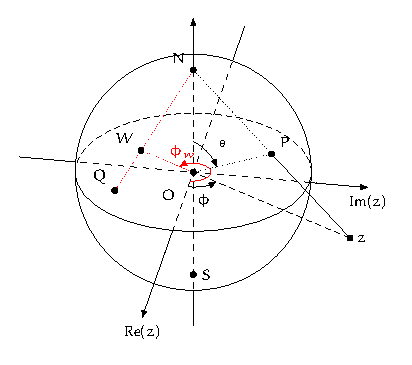
\includegraphics[width=7cm]{images/riemann_sphere.pdf}
\end{center}
To determine analyticity at $\infty$, we set $\zeta = \frac{1}{z}$, and analyze the analyticity of $\tilde{w}\left(\zeta\right) = w\left(1/z\right)$ at $0$.
\subsubsection{Cauchy's Integral Formula}%
Consider the function $w(z) = c/z$, integrated around a circle of radius $R$.
\begin{align*}
  \oint_{\Gamma}w(z)\:dz &= C\int_{0}^{2\pi} \frac{e^{-i\varphi}}{R}\underbrace{iRe^{i\varphi}\:d\varphi}_{dz}\\
                         &= ic\int_{0}^{2\pi} \:dz\\
                         &= 2\pi i c.
\end{align*}
\end{document}
